\documentclass[a4paper]{article}
\usepackage[utf8]{inputenc}
\usepackage{tkz-graph}
\usepackage{titling}
\usepackage{xpatch}
\usepackage{hyperref}
\usepackage[portuguese,english]{babel}
\title{CodeWarriors - Secure Personal Cloud}
\author{170050018(33\%), 170050088(33\%), 170100091(33\%)}
\date{October 23, 2018}

\begin{document}

\setlength\parindent{1cm}

\maketitle
\hfill\begin{minipage}{\dimexpr\textwidth-1cm}
\centerline{ \textbf{Declaration}}
 I acknowledge and understand that plagiarism is wrong. This project is my own
work, or my group’s own unique group project. I acknowledge that copying some-
one else’s work, or part of it, is wrong, and that submitting identical work to others constitutes a form of plagiarism.
\end{minipage}

\section{Work Done so far}

We have researched enough to get broad idea of things to do - particularly how the communication will take place between the clients and server, and thus, how the work can be parallelised effectively.

\noindent We have set up the login and registration pages\cite{login}. The linux client is able to login via the terminal\cite{linux-client-login}. Communication is possible using curl.

\section{System Architecture using TikZ}
\tikzset{
  VertexStyle/.append style = { rectangle, draw
  %,inner sep=5pt
  }
  }
\begin{tikzpicture}
  \SetGraphUnit{5}
  \Vertex{Client}
  \SOWE(Client){Server}
  \SOEA(Client){Database}
  \tikzset{EdgeStyle/.append style = {->,bend left = 20}}
  \Edge(Server)(Client)
  \Edge(Client)(Server)
  \Edge(Server)(Database)
  \Edge(Database)(Server)
\end{tikzpicture}

\section{Results and Analysis}
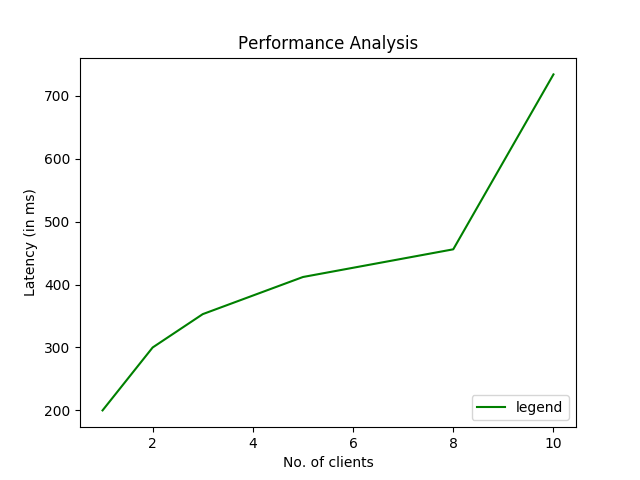
\includegraphics[width=1\textwidth]{plot1.png} \\
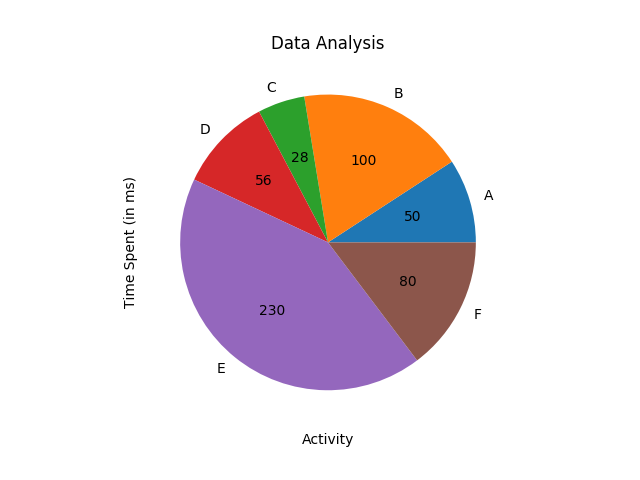
\includegraphics[width=1\textwidth]{plot2.png}

\section{Future Work}
 We plan to use openssl for encryption and decryption on the linux client. For the web client, although cryptojs is a popular library, we have been unable to get it to work so far (in fact, this consumed a major chunk of our time).
 
 \noindent We intend to implement block level encryption by using the bash commands either dd or split. Each of the encrypted blocks will be stored in the database as a row, along with other meta data associated with the data, such as file name, file type, access rights, etc.

\begin{thebibliography}{}
\bibitem{login}
\url{https://wsvincent.com/django-user-authentication-tutorial-login-and-logout/}
\bibitem{linux-client-login}
\url{https://stackoverflow.com/questions/21306515/how-to-curl-an-authenticated-django-app}
\end{thebibliography}

\end{document}
 
